% Full instructions available at:
% https://github.com/elauksap/focus-beamertheme

\documentclass[9pt]{beamer}
\usetheme{focus}

%%%%%%%%%%%%%%%%%%%%%%%%%%%%%%%%%%%%%%%%%%%%%%%%%%%%%%%%%%%%%%%%%%%%%
% Typography, change document font
\usepackage[tt=false, type1=true]{libertine}
\usepackage[varqu]{zi4}
\usepackage[libertine]{newtxmath}
\usepackage[T1]{fontenc}

\usepackage[protrusion=true,expansion=true]{microtype}

% Disable paragraph indentation, and increase gap
\usepackage{parskip}

%Matrix
\usepackage{tabstackengine}
\setstackEOL{;}% row separator
\setstackTAB{,}% column separator
\setstacktabbedgap{1ex}% inter-column gap 
\setstackgap{L}{1.0\normalbaselineskip}% inter-row baselineskip
\let\mat\bracketMatrixstack

\newcommand{\pth}{Figure/}
\newcommand{\ve}[1]{\mathbf{#1}}

% Copyright (C) 2018-2019 Pasquale Claudio Africa and the LaTeX community.
% A full list of contributors can be found at
%
%     https://github.com/elauksap/focus-beamertheme
% 
% This file is part of beamerthemefocus.
% 
% beamerthemefocus is free software: you can redistribute it and/or modify
% it under the terms of the GNU General Public License as published by
% the Free Software Foundation, either version 3 of the License, or
% (at your option) any later version.
% 
% beamerthemefocus is distributed in the hope that it will be useful,
% but WITHOUT ANY WARRANTY; without even the implied warranty of
% MERCHANTABILITY or FITNESS FOR A PARTICULAR PURPOSE. See the
% GNU General Public License for more details.
% 
% You should have received a copy of the GNU General Public License
% along with beamerthemefocus. If not, see <http://www.gnu.org/licenses/>.

\mode<presentation>


% DEFINE COLORS. ---------------------------------------------------------------
\definecolor{main}{RGB}{134, 161, 174}
\definecolor{main2}{RGB}{104, 131, 144}
\definecolor{textc}{RGB}{20, 20, 20}
\definecolor{background}{RGB}{255, 255, 255}

\definecolor{alert}{RGB}{180, 0, 0}
\definecolor{example}{RGB}{0, 110, 0}


% SET COLORS. ------------------------------------------------------------------
\setbeamercolor{normal text}{fg=textc, bg=background}
\setbeamercolor{alerted text}{fg=textc}
\setbeamercolor{example text}{fg=textc}

\setbeamercolor{titlelike}{fg=background, bg=main}
\setbeamercolor{frametitle}{parent={titlelike}}

\setbeamercolor{footline}{fg=background, bg=main2}

\setbeamercolor{block title}{bg=main!80!background, fg=background}
\setbeamercolor{block body}{bg=main!10!background, fg=textc}

\setbeamercolor{block title alerted}{bg=alert, fg=background}
\setbeamercolor{block body alerted}{bg=alert!10!background, fg=textc}

\setbeamercolor{block title example}{bg=example, fg=background}
\setbeamercolor{block body example}{bg=example!10!background, fg=textc}

\setbeamercolor{itemize item}{fg=textc}
\setbeamercolor{itemize subitem}{fg=textc}

\setbeamercolor{enumerate item}{fg=textc!70!black}
\setbeamercolor{enumerate subitem}{fg=textc!70!black}

\setbeamercolor{description item}{fg=textc!70!black}
\setbeamercolor{description subitem}{fg=textc!70!black}

\setbeamercolor{caption name}{fg=textc}

\setbeamercolor{section in toc}{fg=textc}
\setbeamercolor{subsection in toc}{fg=textc}
\setbeamercolor{section number projected}{bg=textc}
\setbeamercolor{subsection number projected}{bg=textc}

\setbeamercolor{bibliography item}{fg=main}
\setbeamercolor{bibliography entry author}{fg=main!70!black}
\setbeamercolor{bibliography entry title}{fg=main}
\setbeamercolor{bibliography entry location}{fg=main}
\setbeamercolor{bibliography entry note}{fg=main}

\mode<all>


\begin{document}
\tableofcontents	
	\section{Surfaces : \today}
	\begin{frame}{First fundamental form}
		\begin{itemize}
			\item Every surface S  can be written as a function of two points $\xi_1$ and $\xi_2$, where we get
			\begin{equation}
			x_1 = f_1(\xi_1,\xi_2) \qquad y = f_2(\xi_1,\xi_2)\qquad z = f_3(\xi_1,\xi_2)
			\end{equation}
			where all the functionsa re single valued continuous functions of $\xi_1,\xi_2$ (Which are called curvilinear coordinates of the surface). By finxing one and changing the other, we get a family of curves called parameteric curves on the surface.
			% TODO: \usepackage{graphicx} required 
			\begin{figure}
				\centering
				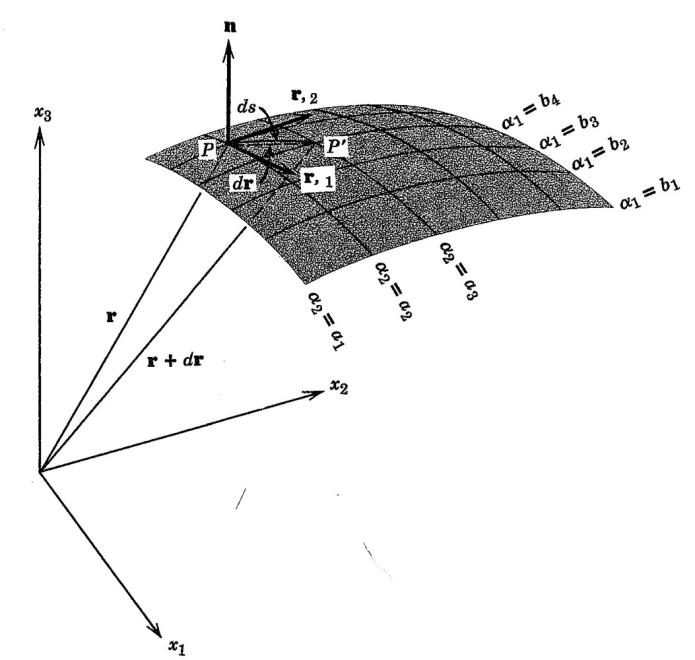
\includegraphics[width=0.5\linewidth]{ fig1}
				\caption{PATH NOT PROPER}
				\label{fig:fig1}
			\end{figure}
			
 		\end{itemize}	
 	\end{frame}


	\begin{frame}
		\begin{itemize}
			\item Now the position of a point on the curve is given as $\ve{r(\xi_1,\xi_2) = f_1(\xi_1,\xi_2)\ve{e_1} +f_2(\xi_1,\xi_2)\ve{e_2} + f_3(\xi_1,\xi_2)}\ve{e_3}$
			\item Now a small differential change d$\ve{r}$ in the vector $\ve{r}$ as we move from a point P to avery close point P' on the surface S can be found as
			\begin{equation}
			d\ve{r} = \frac{\partial \ve{r}}{\partial \xi_1}d\xi_1 + \frac{\partial \ve{r}}{\partial \xi_2}d\xi_2
			\end{equation}
			where we can also write $\ve{r}_{,i} = \frac{\partial \ve{r}}{\partial \xi_i}$ with i =1,2 \\
			for partial derivatives of vectors. The square of the magnitude of the differential change vector $d\ve{r}$ is found by taking the scalar product of d$\ve{r}$ with itself

			\begin{equation}
			\begin{aligned}
				(ds)^2 = d\ve{r} \cdot d\ve{r} =\ve{r}_{,1}\cdot \ve{r}_{,1} (d\xi_1)^2 +\ve{r}_{,1}\cdot \ve{r}_{,2} (d\xi_1)(d\xi_2)+\ve{r}_{,2}\cdot \ve{r}_{,2} (d\xi_2)^2\\
				 = E (d\xi_1)^2 + F(d\xi_1)(d\xi_2)+G(d\xi_2)^2
			\end{aligned}	
			\end{equation}
			which is the fundamental form of the surface by knowing the fundamental magnitudes E,F,G. 
			\item We note that $\ve{r}_{,i}$ are the tangents to the curves of constant $\xi_1,\xi_2$. F will be zero if the paremetric curves form an orthogonal net. We can write it also as
			\begin{equation}
			(ds)^2 = A_1^2 (d\xi_1)^2  + A_2^2  (d\xi_2)^2 
			\end{equation}
			where $A_1 = \sqrt{E},\quad A_2 = \sqrt{G}$
		\end{itemize}
	\end{frame}


	\begin{frame}{Normal to a surface}
		\begin{itemize}
			\item At every point P, there exists a unit normal vector $\ve{n(\xi_1,\xi_2)}$	 which is perpendicular to $\ve{r}_{,1},\ve{r}_{,2}$  and hence to the tangent plane at P. We get n by the familiar expression
			\begin{equation}
				\ve{n(\xi_1,\xi_2)}= \ve{r,_1} \times \ve{r,_2} / | \ve{r,_1} \times \ve{r,_2} |
			\end{equation}
			where we have 
			\begin{equation}
			\begin{aligned}
			| \ve{r,_1} \times \ve{r,_2} | = | \ve{r,_1}|| \ve{r,_2} | sin\theta \\
			 \ve{r,_1} \cdot \ve{r,_2}  = | \ve{r,_1}|| \ve{r,_2} | cos\theta
			\end{aligned}
			\end{equation}
			and we have expressions by manipulation : $ cos \theta = F/\sqrt{EG}, \quad sin \theta = \sqrt{(EG-F^2)/EG} = H/\sqrt{G}$. We can also have $\ve{n(\xi_1,\xi_2)}= \ve{r,_1} \times \ve{r,_2} / H$ provided H does not vanish
			\item The principal normal $N$ does  not need to be normal to the surface ($\ve{N.n}$ $\neq$ 1)
			
		\end{itemize}
	\end{frame}


	\begin{frame}{Second Fundamental form}
		We have described the curvature vector $\ve{k}$ of a space curve. We shall consider a curve on a surface and use the properties of the curvature vector to derive an important features of surfaces of the second fundamental form
		\begin{itemize}
			\item Recall that the curvature vector $\ve{k}$ is given by $\frac{d\ve{T}}{ds}$ where $\ve{T}$ is the unit vector tangent to the curve.
			\item The curvature vector $\ve{k}$ of the curve into its normal and tangenetial components to the surface. Thus
			\begin{equation}
			\ve{k} = \frac{d\ve{T}}{ds} = \ve{k_n+k_t}
			\end{equation}
			$k_n$ and $k_t$ are the normal and tangential curvature vector.
			\item Since $\ve{k_n}$ is in the direction of the normal to the surface, it is proportional to $\ve{n}$ and can be expressed in terms as
			\begin{equation}
				\ve{k_n} = - K_n \ve{n}
			\end{equation}
			The minus sign takes into account the fact that the senese of the curvature vector $\ve{k}$ is opposite to that of the normal vector $\ve{n}$
		\end{itemize}
	\end{frame}


	\begin{frame}{Curvature of surface}
		\begin{itemize}
			\item Since $\ve{n}$ is perpendicular to $\ve{T}$, differentiation with respect to s along the surface gives
			\begin{equation}
			\frac{d \ve{n}}{ds} \cdot \ve{T} = -\ve{n}\cdot \frac{d \ve{T}}{s}
			\end{equation}
			\item If we form the scalar of $\ve{k_n =} -K_n \ve{n}$, where $K_n$ , we get
			\begin{equation}
			-(\ve{k_n}\cdot n) = K_n
			\end{equation}
			\item And finally we will get 
			\begin{equation}
			K_n = \frac{d\ve{r}\cdot d\ve{n}}{d\ve{r}\cdot d\ve{r}}
			\end{equation}
			where we use\\
			$(ds)^2 = d\ve{r}\cdot d\ve{r}$, now if we keep \\ 
			$d\ve{n} = \ve{n,_1}d\xi_1 + \ve{n,_2}d\xi_2$ \\
			$d\ve{r} = \ve{r,_1}d\xi_1 + \ve{r,_2}d\xi_2$
			\begin{equation}
			K_n = \frac{II}{I} = \frac{L (d\xi_1)^2 + 2M (d\xi_1d\xi_2) + N (d\xi_2)^2}{E (d\xi_1)^2 + 2F (d\xi_1d\xi_2) + G (d\xi_2)^2}
			\end{equation}
			where $L = \ve{r,_1 \cdot n,_1} \qquad 2M = \ve{r,_1 \cdot n,_2 + r,_2 \cdot n,_1 } \qquad L = \ve{r,_2 \cdot n,_2}$
		\end{itemize}
	\end{frame}


	\begin{frame}{Principal curves}
		\begin{itemize}
			\item Now since we have the principal curvatures, we want to find the direction ($\alpha = d\xi_1/d\xi_2$) for which the normal curvature $K_n$ has a maximum or minimum force. 
			\item We then get the curvature as
			\begin{equation}
			K(\alpha) = \frac{L + 2M \lambda + N\lambda^2}
			                 {E + 2F \lambda + G\lambda^2}
			\end{equation}
			\item The curvature attains an extremum in some direction $\lambda$ if $\frac{dK}{d\lambda} = 0$
			\item Solving the quadratic equation will result into two roos corresonding to the two directions ($d\xi_1/d\xi_2)_1$ and ($d\xi_1/d\xi_2)_2$ of
			\begin{equation}
			(MG-NF)\lambda^2 + (LG-NE)\lambda + (LF-ME)  = 0
			\end{equation}
			One solution is the maximum while the other is the minimum curvature
		\end{itemize}
	\end{frame}


	\begin{frame}{Principal curves}
		\begin{itemize}
			\item Now $K_1 =1/R_1 \quad K_2 =1/R_2$ are called principal curces.
			\item These two are actually orthogonal and it can be proven (Check Harry Kraus)
			\item Suppose the lines of curvature are taken as the parametric lines. Therefore $d\xi_1/d\xi_2 = 0$ and $d\xi_2/d\xi_1 = 0$ should statisfy the eigen value problem
			\item It will come out that F =  M = 0 and we can get
			\begin{equation}
			 K_1 = 1/R_1 = L/E \qquad K_2 = 1/R_2 = N/G
			\end{equation}
		\end{itemize}
	\end{frame}


	\begin{frame}{Derivatives of unit vectors along parametric lines}
		\begin{itemize}
			\item Consider a triplet of orthogonal unit vectors ($\ve{t_1,t_2,n}$) so that they are thangent to $\xi_1,\xi_2$ and normal to the surface respectively.
			\item As we move on the surfcace, we end up changing the orientation of these unit vector, bu they remain constant at unity and orthogonal
			\item Let us firstly define these vectors
			\begin{equation}
			\begin{aligned}
			\ve{t_1 = \frac{r,_1}{\ve{|r,_1|}}} \\
			\ve{t_2 = \frac{r,_2}{\ve{|r,_2|}}} \\
			\ve{n = t_1 \times t_2} \\
			\end{aligned}
			\end{equation}
			
		\end{itemize}
	\end{frame}


	\begin{frame}{Derivatives of normal along parametric lines}
		\begin{itemize}
			\item Interesting thing is that since $\ve{n,_1}$ and $\ve{n,_2}$ are prependicular to $\ve{n}$, they lie in the plane formed by $\ve{t_1}$ and $\ve{t_2}$. Therefore we can decompose like $\ve{n,_1} =  a \ve{t_1} + b \ve{t_2}$
			\item To find $a,b$ we dot product with $\ve{t_1,t_2}$ to get two equations
			\item Since the system is orthogoanl M = $\ve{t_1\cdot t_2} = 0$
			\begin{equation}
			a = \frac{L}{A_1} \qquad b = 0
			\end{equation}			
			\item  And interstingly we get that it is in the direction of the tangents itself given as 
			\begin{equation}
			\begin{aligned}
				\ve{n,_1} = \frac{A_1}{R_1}\ve{t_1} \\				\ve{n,_2} = \frac{A_2}{R_2}\ve{t_1} \\
			\end{aligned}
			\end{equation}
			So we have found the derivatives of the normal along the parametric lines.
		\end{itemize}
	\end{frame}


	\begin{frame}{Derivative of tangent along parametric lines}
		\begin{itemize}
			\item To find the derivatives of $\ve{t_1,t_2}$ along the parmetric lines we proceed as we did for the case of the derivatives of $\ve{n}$
			\item For continuous with continuous second derivatives we get $\ve{r,_{12} }= \ve{r,_{21} }$ allowing us to write
			\begin{equation}
			\begin{aligned}
				(A_1t_1),_2 = (A_2t_2),_1 \\
				\ve{t_2,_1} = \frac{1}{A_2} [A_1\ve{t_1,_2} 
				+ A_1,_2\ve{t_1} - A_2,_1\ve{t_2}]
			\end{aligned}
			\end{equation}
			\item As state we want to find $\ve{t_1,_1} \quad \ve{t_1,_2}$
			\item We observe that this derivative will be perpendicular to $\ve{t_1}$ and will lie in the plane formed by $\ve{t_2}$ and $\ve{n}$. We can therefore express it as 
			\begin{equation}
			  \ve{t_1,_1} = c \ve{n} + d \ve{t_2}
			\end{equation}
			where we can find c and d by finding the dot product with $\ve{n}$ and $\ve{t_2}$
			\item We then get
			\begin{equation}
			\begin{aligned}
				\ve{t_1,_1} = -\frac{ A_1}{R_1}\ve{n} - \frac{1}{A_2}A_1,_2 \ve{t_2}
			\end{aligned}
			\end{equation}
			Other directions, you can find from Harry Kraus
		\end{itemize}
	\end{frame}

	\begin{frame}{Gauss Codazzi conditions}
		\begin{itemize}
			\item The first condition is 
			\begin{equation}
			\frac{1}{R_1}A_1,_2 = \left(\frac{A_1}{R_1} \right)_{,2} \qquad,
			\frac{1}{R_2}A_2,_2 = \left(\frac{A_2}{R_2} \right)_{,1}
			\end{equation}
			\item The other is
			\begin{equation}
			\left(\frac{1}{A_1}A_{2,1} \right)_{,1}
			+
			\left(\frac{1}{A_2}A_{1,2} \right)_{,2} 
			= -\frac{A_1A_2}{R_1R_2}
			\end{equation}
			\item If E,G,L and N are given as funcions of the real curvilinear coordinates $\xi_1,\xi_2$ and are sufficiently differentialbe and satisfy Gauss codazzi equations wile E>0 and G>0. Then there exist a real surface with 1 and 11 form as
			\begin{equation}
			I = E(d\xi_1)^2 + G(d\xi_2)^2 \qquad II =  L(d\xi_1)^2 + N(d\xi_2)^2 
			\end{equation}
			\item This is for the simplified cases where the lines of principle curvature are the parametric lines (F=M=0). Now more general Gauss Codazzi equations also exist.
		\end{itemize}
	\end{frame}


	\begin{frame}{Example: Surface of revolution}
		\begin{itemize}
			\item Suppose that there is a srface which is given as 
			\begin{equation}
			\ve{r}(x_3,\theta) = R_o(x_3)cos\theta \ve{e_1} + R_o(x_3)sin\theta \ve{e_2} + x_3\ve{e_3}
			\end{equation}
			\item Now in finding $g$ we get, keeping $x_3,\theta$ as $\xi_1$ and $\theta$ as $\xi_2$, we get:
			\begin{equation}
			\begin{aligned}
			\frac{d \ve{r}}{d\xi_1} = \ve{r},_1 = R_o'(x_3)cos\theta \ve{e_1} + R_o'(x_3)sin\theta \ve{e_2} + \ve{e_3} \\ 
			\frac{d \ve{r}}{d\xi_2} = \ve{r},_2 = -R_o(x_3)sin\theta \ve{e_1} + R_o(x_3)cos\theta \ve{e_2} + 0\ve{e_3} \\ 
			\end{aligned}
			\end{equation}
		\end{itemize}
	\end{frame}


	\begin{frame}{Fundamental forms -I}
		\begin{itemize}
			\item E = $\ve{r},_1 \cdot \ve{r},_1 
			= R_o^{2'}cos^2\theta+ R_o^{2'}sin^2\theta + 1 = 1 + R_o^{2'}$
			\item F =  $\ve{r},_1 \cdot \ve{r},_2 =  -R_o^2cos\theta sin\theta + R_o^2cos\theta sin\theta = 0$
			\item  G =   $ \ve{r},_2 \cdot \ve{r},_2 = R_o^2sin^2\theta+ R_o^2cos^2\theta  =  R_o^2$
			\item H = $\sqrt{EG-F^2} = R_o\sqrt{1+R_o^{2'}}$
			\item $A_1 = \sqrt{E} \qquad A_2 = \sqrt{G}$
			\item First form : $(ds)^2 = \left(1 +   R_o^{2'}\right)dx_3^2 + R_o^2 d\theta^2$
			\item Normal to surface $\ve{n} = \frac{\ve{r},_1\times \ve{r},_2}{H} = \frac{-R_o}{H} \left(cos \theta \ve{e_1}
			+ sin \theta \ve{e_1} -  R_o' \ve{e_3}\right)$ 
			\\ It acts as assumed from conncave to convex side
		\end{itemize}
	
	\end{frame}


	\begin{frame}{Fundamental forms - II}
		\begin{itemize}
			\item $L = - \ve{r},_{11}\cdot \ve{n} = \frac{-R_o}{H} \mat{R_o''cos\theta , R_o''sin\theta,0} \cdot \mat{cos \theta; sin \theta; -R_o'} = -R_oR_oH''/H$
			\item M = $-\ve{r},_{12} = 0 $
			\item N = $-\ve{r},_{22} =  R_o^2/H$
			\item Principal curvatures $R_1 = E/L \quad R_2 = G/N$
			\item We can check the gauss codazzi to test the surface
			\item An alternate description is if we use $\phi,\theta$ where the first is the angle between the axis revolution of the surface and a normal to the surface of the point. (See Kraus)
		\end{itemize}
	\end{frame}

\end{document}